\subsection{Introduction}

The team decided it would be in the best interests of the application if we had real world data and enough of it to properly test the capabilities of the algorithm and thus therefore allowing there to be sufficient enough reason to have a GUI as, without much data, say if it was instead a small amount of hard-coded data then the GUI would've ended up much more basic. With that decision came finding a reliable source of baseball match information for an entire season and so we decided to use the match listings from x. The process unfortunately involved a lot of manual copy and pasting due to the formatting and structure of the information on the website with at most only two days worth of matches being shown on the same page. 

Eventually the source file after having the entire seasons match line up and information appended continually to it, was finished but still had unnecessary columns. This was solved by taking the source file, placing it into Microsoft Excel, selecting the entire redundant columns and simply removing them leaving only the relevant information. This, along with a few tweaks to get rid of hidden characters taken from the formatting of the website left us with a reliable source of Baseball's entire 2012 season information to pass into the program.

The reasoning behind using 2012's season information was because we discovered at the start of the project, the season was just finishing as it had ran since April and it wouldn't be starting again until April 2013. This meant that it wouldn't run throughout the same time frame we would have to complete the project which if it had would've allowed us to actively, in real time update the system day by day as the results of matches were published. This was the main reasoning behind the teams decision in the second semester to instead drop the future work plan of creating a web based parser that would've made use of some variation of an RSS feed or an HTML page to extract recent match information continually. 

There was no time overlap to allow real data to be parsed so we looked into using the next closest sport in terms of the point system; Basketball due to it having a season running alongside the project time frame in part. The team ultimately decided to throw this out due to small discrepancies that made it less viable to use such as 2-1-0 point scoring instead of Baseballs 1-0, not to mention that a lot of time would be spent making the parser come to fruition when we could use the time to make more features within the desktop application and ultimately the creation of the web application.

Regardless these were the main reasons behind the teams decision to instead work retrospectively over a finished season; it allowed us to know the conclusions for the end of season scores showing that the algorithm did in fact truly work when it was completed due to the data matching up and it also allowed the application to test an entire season right from the beginning to check it's speed capabilities with a full data set.

\subsection{Design}
The design of the parser required figuring out which classes needed to be created in order to pass information to the algorithm and the user interface, essentially the backbone of the entire application. Once these were established and implemented the match information was to flow externally from a specifically structured source text file, user specified or 2012's default season otherwise. Once the information had been sucessfully read in, parsed and stored it would populate the main classes within the program and could be used by either the algorithm or the user interface whenever required. The other task was to make more functionality within the main classes such that the coding by the other components could be simplified to function calls as extra functionality would exist to support them.

\subsection{Implementation}

The main classes were identified as Divison, Match and Team with the Parser class being metaphorical funnel that pours information into these classes. Initially starting out by scanning line by line the provided source file until it reaches the end having created appropriate objects and stored the relevant information during the process.

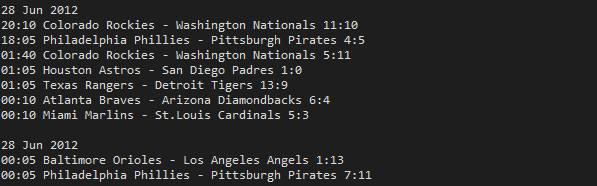
\includegraphics[width=\linewidth,keepaspectratio]{images/sourceFileExample.png}

As can be seen in the screenshot above this is a sample of data from the 2012 source file. The structure of each line below the date is as follows;
 
\begin{verbatim}
Time 	Hometeam - Awayteam 	Home Score:Away Score
\end{verbatim}

The parser will determine whether it's on a new date or a match and dependant on which will call the appropriate function that will go a layer deeper and perform string manipulation to split apart, analyse each individual piece, store and/or create objects for in the appropriate classes before finishing up and moving onto the next line in the file should it be a new date or match.

To go more in-depth, the parser must first initialise the 6 available Baseball divisions that exist such as "American Central" or "National West", by manually hard-coding their names and the names of the 5 teams associated with each division because there is no other way to set up the divisions automatically from an external source. These populated division objects along with the team objects are stored together in a easily accessible hash map and from here the parser moves onto it's main functionality as shown by the following pseudocode;

\begin{verbatim}
			Match Information
1. While there are still more lines in the source
	1.1 split the current line by whitespace into an array 
	1.2 determine if it's a match or date line based on length and call appropriate function
2. Initialise variables
	2.1 split time since it's always first element into array
	2.2 split score since it's always last element into array
3. If the score array has 2 elements
	3.1 store each in a separate home or away int variable
	3.2 set the match to played
4. Loop through the next element after time
	4.1 append each letter to first team name
5. Loop through the second last element
	5.1 append each letter to second team name
6. Link newly created team objects to the already initialised ones in the division's object using the extracted team name as the link.
7. Error check the link was successful and that the match has scores.
8. Create a match object populating it with all the variables/objects created above
9. Set both the home/away teams upcoming matches with that match object
10. Add that match object to the list of league fixtures
\end{verbatim}

\begin{verbatim}
			Date Information
1. While there are still more lines in the source
	1.1 split the current line by whitespace into an array 
	1.2 determine if it's a match or date line based on length and call appropriate function
2. Store first element as day, third as year
	2.1 create a new date object using the 3 elements to specify the date
\end{verbatim}
